\chapter{Projekt bazy danych}
\label{ch:baza_danych}

Właściwe zaplanowanie bazy danych stanowiło fundament systemu, od którego zależała wydajność i poprawność przechowywania kluczowych informacji. Baza danych zaprojektowana dla systemu Rock Gym została oparta o relacyjny model danych i zaimplementowana w technologii MySQL.

\section{Opis modelu danych i diagram ERD}

Struktura bazy danych została odwzorowana na schemacie w postaci diagramu ERD(rys. \ref{fig:erd_diagram}), który przedstawia poszczególne tabele, ich atrybuty oraz zachodzące między nimi relacje.

\begin{figure}[H]
    \centering
    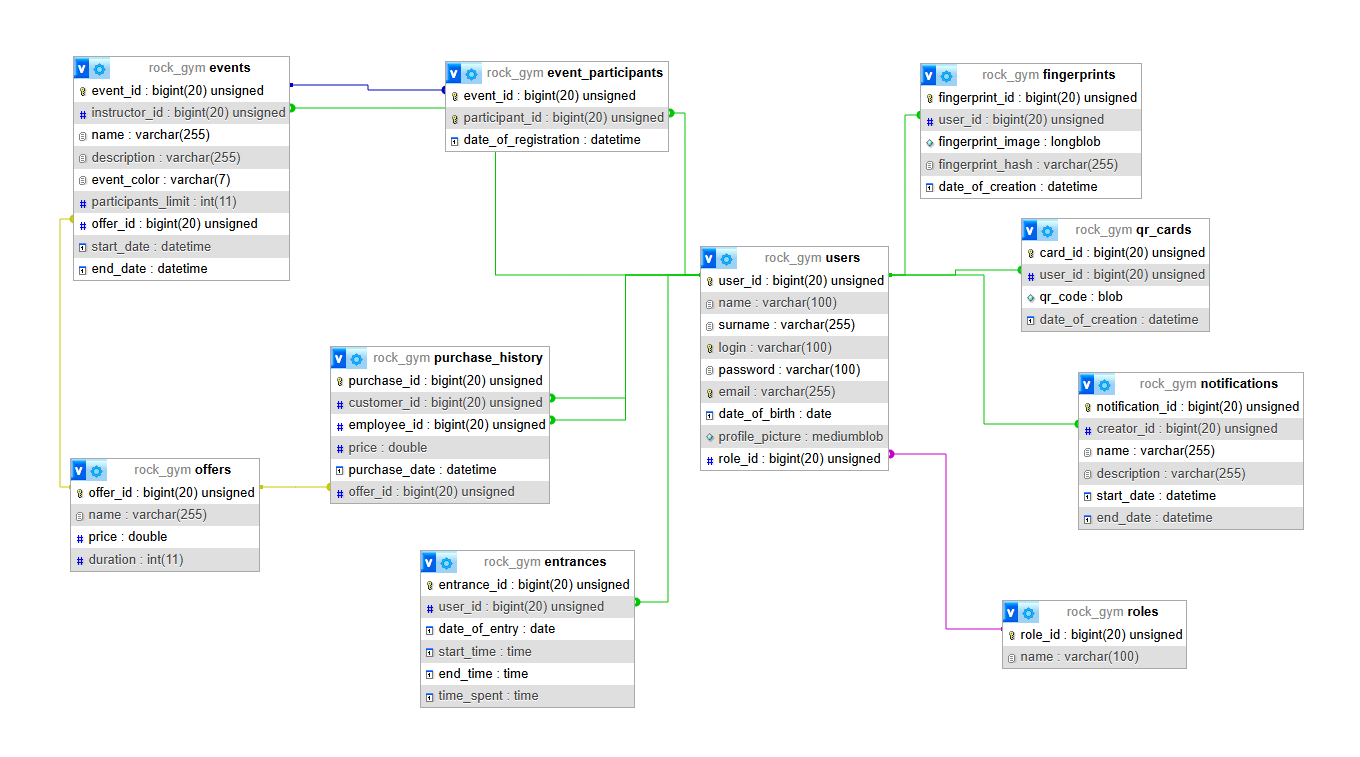
\includegraphics[width=0.9\textwidth]{figures/erd.png}
    \caption{Diagram ERD bazy danych systemu Rock Gym}
    \label{fig:erd_diagram}
\end{figure}


Poniżej rozpisano szczegółowy opis struktury wszystkich tabel w bazie danych.

\noindent\textbf{Tabela entrances:} Tabela przechowuje historię wejść i wyjść użytkowników z obiektu.
\begin{itemize}[noitemsep, topsep=0pt]
    \item \texttt{entrance\_id} -- unikalny identyfikator wejścia, pełniący funkcję klucza głównego.
    \item \texttt{user\_id} -- klucz obcy powiązany z identyfikatorem użytkownika dokonującego wejścia.
    \item \texttt{date\_of\_entry} -- data wejścia użytkownika.
    \item \texttt{start\_time} -- godzina rozpoczęcia wizyty.
    \item \texttt{end\_time} -- godzina zakończenia wizyty na ściance.
    \item \texttt{time\_spent} -- całkowity czas spędzony na ściance podczas danej wizyty.
\end{itemize}

\noindent\textbf{Tabela events:} Tabela zawiera informacje o zaplanowanych wydarzeniach, zajęciach oraz kursach.
\begin{itemize}[noitemsep, topsep=0pt]
    \item \texttt{event\_id} -- unikalny identyfikator wydarzenia będący jego kluczem głównym.
    \item \texttt{instructor\_id} -- klucz obcy powiązany z identyfikatorem instruktora prowadzącego zajęcia.
    \item \texttt{name} -- nazwa wydarzenia.
    \item \texttt{description} -- opis zaplanowanego wydarzenia.
    \item \texttt{event\_color} -- kod koloru używany do wyświetlania wydarzenia w kalendarzu.
    \item \texttt{participants\_limit} -- maksymalna liczba uczestników wydarzenia.
    \item \texttt{offer\_id} -- klucz obcy wskazujący na ofertę powiązaną z wydarzeniem.
    \item \texttt{start\_date} -- data i godzina rozpoczęcia wydarzenia.
    \item \texttt{end\_date} -- data i godzina zakończenia wydarzenia.
\end{itemize}

\noindent\textbf{Tabela event\_participants:} Tabela asocjacyjna określająca zapisy użytkowników na poszczególne wydarzenia.
\begin{itemize}[noitemsep, topsep=0pt]
    \item \texttt{event\_id} -- klucz obcy będący częścią klucza głównego, powiązany z wydarzeniem.
    \item \texttt{participant\_id} -- klucz obcy będący częścią klucza głównego, powiązany z identyfikatorem użytkownika biorącego udział w wydarzeniu.
    \item \texttt{date\_of\_registration} -- data i czas rejestracji uczestnika na dane wydarzenie.
\end{itemize}

\noindent\textbf{Tabela fingerprints:} Tabela przechowująca dane biometryczne klientów w postaci wzorców odcisków palców.
\begin{itemize}[noitemsep, topsep=0pt]
    \item \texttt{fingerprint\_id} -- unikalny identyfikator rekordu biometrycznego (klucz główny).
    \item \texttt{user\_id} -- klucz obcy powiązany z identyfikatorem użytkownika, do którego przypisany jest odcisk palca.
    \item \texttt{fingerprint\_image} -- przetworzony obraz odcisku palca.
    \item \texttt{fingerprint\_hash} -- wyekstraktowany z obrazu wzorzec biometryczny, służący do szybkiego porównywania odcisku.
    \item \texttt{date\_of\_creation} -- data dodania i zapisania odcisku w bazie danych.
\end{itemize}

\noindent\textbf{Tabela notifications:} Tabela zawiera informacje o powiadomieniach kierowanych do użytkowników, wyświetlanych np. w aplikacji.
\begin{itemize}[noitemsep, topsep=0pt]
    \item \texttt{notification\_id} -- unikalny identyfikator powiadomienia pełniący funkcję klucza głównego.
    \item \texttt{creator\_id} -- klucz obcy wskazujący na użytkownika (pracownika, menadżera), który utworzył powiadomienie.
    \item \texttt{name} -- tytuł powiadomienia.
    \item \texttt{description} -- treść powiadomienia.
    \item \texttt{start\_date} -- data i godzina rozpoczęcia widoczności powiadomienia.
    \item \texttt{end\_date} -- data i godzina zakończenia widoczności powiadomienia.
\end{itemize}

\noindent\textbf{Tabela offers:} Tabela określająca cennik i ofertę obiektu sportowego (np. karnety, jednorazowe wejścia).
\begin{itemize}[noitemsep, topsep=0pt]
    \item \texttt{offer\_id} -- unikalny identyfikator oferty stanowiący jej klucz główny.
    \item \texttt{name} -- nazwa oferowanej usługi lub karnetu.
    \item \texttt{price} -- cena przypisana do danej pozycji z oferty.
    \item \texttt{duration} -- czas ważności lub trwania danej usługi wyrażony w dniach.
\end{itemize}

\noindent\textbf{Tabela purchase\_history:} Tabela przechowująca historię wszystkich transakcji i zakupów dokonanych przez klientów.
\begin{itemize}[noitemsep, topsep=0pt]
    \item \texttt{purchase\_id} -- unikalny identyfikator przeprowadzonej transakcji (klucz główny).
    \item \texttt{customer\_id} -- klucz obcy wskazujący na klienta dokonującego zakupu.
    \item \texttt{employee\_id} -- klucz obcy wskazujący na pracownika potwierdzającego transakcję.
    \item \texttt{price} -- kwota, za jaką została sprzedana dana oferta w momencie transakcji.
    \item \texttt{purchase\_date} -- dokładna data i czas dokonania transakcji zakupu.
    \item \texttt{offer\_id} -- klucz obcy powiązany ze sprzedaną ofertą z cennika.
\end{itemize}

\noindent\textbf{Tabela qr\_cards:} Tabela przechowująca kody QR przypisane użytkownikom używane jako alternatywna metoda weryfikacji.
\begin{itemize}[noitemsep, topsep=0pt]
    \item \texttt{card\_id} -- unikalny identyfikator karty QR pełniący funkcję klucza głównego.
    \item \texttt{user\_id} -- klucz obcy powiązany z użytkownikiem posiadającym przypisaną kartę QR.
    \item \texttt{qr\_code} -- wygenerowany obraz kodu QR przypisanego do konta.
    \item \texttt{date\_of\_creation} -- data wygenerowania i dodania kodu QR.
\end{itemize}

\noindent\textbf{Tabela roles:} Tabela definiująca możliwe role i poziomy uprawnień w systemie.
\begin{itemize}[noitemsep, topsep=0pt]
    \item \texttt{role\_id} -- unikalny identyfikator uprawnień będący kluczem głównym.
    \item \texttt{name} -- słowna nazwa roli (admin, pracownik, instruktor, klient).
\end{itemize}

\noindent\textbf{Tabela users:} Tabela zawiera informacje o zarejestrowanych użytkownikach w systemie i dane logowania.
\begin{itemize}[noitemsep, topsep=0pt]
    \item \texttt{user\_id} -- unikalny identyfikator użytkownika będący kluczem głównym tabeli.
    \item \texttt{name} -- imię użytkownika.
    \item \texttt{surname} -- nazwisko użytkownika.
    \item \texttt{login} -- login użytkownik.
    \item \texttt{password} -- hasło użytkownika zabezpieczone przez proces szyfrowania.
    \item \texttt{email} -- unikalny adres email użytkownika.
    \item \texttt{date\_of\_birth} -- data urodzenia zarejestrowanego użytkownika.
    \item \texttt{profile\_picture} -- opcjonalne zdjęcie profilowe użytkownika.
    \item \texttt{role\_id} -- klucz obcy definiujący uprawnienia użytkownika.
\end{itemize}

\section{Relacje, klucze i normalizacja bazy danych}

Baza danych systemu Rock Gym została zaprojektowana zgodnie z zasadami trzeciej postaci normalnej (3NF). Pozwala to uniknąć powielania informacji i zapewnia spójność logiczną. Każda tabela posiada klucz główny, najczęściej w postaci automatycznie inkrementowanego identyfikatora.

Relacje między tabelami są realizowane za pośrednictwem kluczy obcych. Występujące powiązania między tabelami przedstawiono poniżej:

\begin{itemize}
    \item Relacja 1:N \texttt{users.role\_id > roles.role\_id} \\
          Jedna rola może być przypisana do wielu użytkowników. Natomiast jeden użytkownik posiada tylko jedną przypisaną rolę.

    \item Relacja 1:N \texttt{entrances.user\_id > users.user\_id} \\
          Jeden użytkownik może zarejestrować wiele wejść na obiekt. Natomiast każde wejście należy tylko do jednego użytkownika.

    \item Relacja 1:N \texttt{fingerprints.user\_id > users.user\_id} \\
          Jeden użytkownik może posiadać wiele zapisanych wzorców odcisków palców. Natomiast dany odcisk identyfikuje wyłącznie jednego użytkownika.

    \item Relacja 1:N \texttt{qr\_cards.user\_id > users.user\_id} \\
          Jeden użytkownik może mieć wygenerowanych wiele kodów QR. Natomiast konkretny kod przypisany jest tylko do jednego konta.

    \item Relacja 1:N \texttt{purchase\_history.customer\_id > users.user\_id} \\
          Jeden klient może posiadać wiele transakcji w historii. Natomiast pojedynczy zakup jest powiązany tylko z jednym klientem.

    \item Relacja 1:N \texttt{purchase\_history.employee\_id > users.user\_id} \\
          Jeden pracownik może zatwierdzić wiele transakcji. Natomiast dana transakcja posiada tylko jednego pracownika potwierdzającego.

    \item Relacja 1:N \texttt{purchase\_history.offer\_id > offers.offer\_id} \\
          Pojedyncza oferta może być sprzedana wiele razy. Natomiast dany zakup dotyczy tylko konkretnej oferty.

    \item Relacja 1:N \texttt{events.instructor\_id > users.user\_id} \\
          Jeden instruktor może prowadzić wiele różnych wydarzeń. Natomiast wydarzenie ma tylko jednego głównego prowadzącego.

    \item Relacja 1:N \texttt{events.offer\_id > offers.offer\_id} \\
          Z jedną ofertą może być powiązanych wiele różnych wydarzeń. Natomiast dane wydarzenie jest powiązane z jedną ofertą.

    \item Relacja 1:N \texttt{notifications.creator\_id > users.user\_id} \\
          Jeden pracownik (twórca) może opublikować wiele powiadomień. Natomiast dane powiadomienie przypisane jest do jednego autora.

    \item Relacja M:N (realizowana przez tabelę \texttt{event\_participants}) \\
          Jeden uczestnik może zapisać się na wiele wydarzeń, a w jednym wydarzeniu może brać udział wielu uczestników. Tabela asocjacyjna wykorzystuje klucze obce \texttt{event\_id > events.event\_id} oraz \texttt{participant\_id > users.user\_id}.
\end{itemize}

\section{Integralność danych i migracje}

Zapewnienie bezpieczeństwa oraz ciągłości danych jest jednym z głównych założeń projektowanej bazy. Spójność relacji wspierana jest przez stosowanie reguł ograniczeń obcych kluczy (np. \texttt{ON DELETE CASCADE} lub \texttt{ON DELETE SET NULL}), które dbają o to, by przy usunięciu danego użytkownika z systemu, usunięte zostały również przypisane do niego odciski palców czy kody QR, minimalizując ryzyko wystąpienia niepołączonych danych.

Strukturą bazy danych od strony aplikacji zarządza Entity Framework Core w podejściu \textit{Code-First}. Co oznacza, że wszelkie zmiany w architekturze bazy są realizowane z poziomu kodu w języku C\# przy użyciu mechanizmu migracji. System automatycznie generuje odpowiednie skrypty pozwalające zsynchronizować modele w kodzie z bazą danych, co zapobiega usterkom związanym z niewłaściwym zarządzaniem modelami danych.

\subsection{Bezpieczne przechowywanie danych}

Istotnym aspektem systemu jest obsługa kluczowych informacji, w tym haseł logowania oraz danych biometrycznych. Hasła użytkowników nie są przechowywane otwartym tekstem. W trakcie rejestracji przechodzą przez proces haszowania, wykorzystujący algorytm BCrypt.

W przypadku odcisków palców archiwizowanych w tabeli \texttt{fingerprints}, nie przechowuje się ich wyłącznie jako pliki graficzne w surowej formie do dalszej autoryzacji. Proces pobrania wzorca na urządzeniu skanującym wyciąga z odcisku punkty charakterystyczne i generuje specjalny \textit{hash} autoryzujący użytkownika.
